%        File: defense.tex
%     Created: Sun May 5 10:00 PM 2013 C
%


%\documentclass[11pt,handout]{beamer}
\documentclass[9pt]{beamer}
\usetheme[white]{Wisconsin}
%\title[short title]{long title}
\title[ Thesis Defense ]{ An Integrated Used Fuel Disposition and Generic Repository Model for Fuel Cycle Analysis }
%\subtitle[short subtitle]{long subtitle}
\subtitle[PhD Defense]{PhD Defense}
%\author[short name]{long name}
\author[Kathryn D. Huff]{Kathryn D. Huff}
%\date[short date]{long date}
\date[5.17.2013]{May 17, 2013}
%\institution[short name]{long name}
\institute[UW-Madison]{University of Wisconsin-Madison}

%\usepackage{bbding}
\usepackage{amsfonts}
\usepackage{amsmath}
\usepackage{graphicx}
\usepackage{subfigure}
\usepackage{booktabs} % nice rules for tables
\usepackage{microtype} % if using PDF
\usepackage{bigints}
\newcommand{\units}[1] {\:\text{#1}}%
\newcommand{\SN}{S$_N$}%{S$_\text{N}$}%{$S_N$}%
\DeclareMathOperator{\erf}{erf}

%page numbers
\setbeamertemplate{footline}[page number]
%Those icons in the references are terrible looking
\setbeamertemplate{bibliography item}[text]
\begin{document}
%%%%%%%%%%%%%%%%%%%%%%%%%%%%%%%%%%%%%%%%%%%%%%%%%%%%%%%%%%%%%
%% From uw-beamer Here's a handy bit of code to place at 
%% the beginning of your presentation (after \begin{document}):
\newcommand*{\alphabet}{ABCDEFGHIJKLMNOPQRSTUVWXYZabcdefghijklmnopqrstuvwxyz}
\newlength{\highlightheight}
\newlength{\highlightdepth}
\newlength{\highlightmargin}
\setlength{\highlightmargin}{2pt}
\settoheight{\highlightheight}{\alphabet}
\settodepth{\highlightdepth}{\alphabet}
\addtolength{\highlightheight}{\highlightmargin}
\addtolength{\highlightdepth}{\highlightmargin}
\addtolength{\highlightheight}{\highlightdepth}
\newcommand*{\Highlight}{\rlap{\textcolor{HighlightBackground}{\rule[-\highlightdepth]{\linewidth}{\highlightheight}}}}
%%%%%%%%%%%%%%%%%%%%%%%%%%%%%%%%%%%%%%%%%%%%%%%%%%%%%%%%%%%%%
%%--------------------------------%%
\frame{
  \titlepage
}

\section{Motivation}
%%--------------------------------%%
\begin{frame}
  \frametitle{Outline}
  \tableofcontents[currentsection]
\end{frame}

\subsection{Future Fuel Cycle Options}
\include{fuel_cycle_options}
\subsection{Geologic Disposal Concept Options}


%%----------------------------------------%%
\begin{frame}[ctb!]
  \frametitle{Repository Components}
\footnotesize{
  \begin{figure}[htbp!]
  \begin{center}
    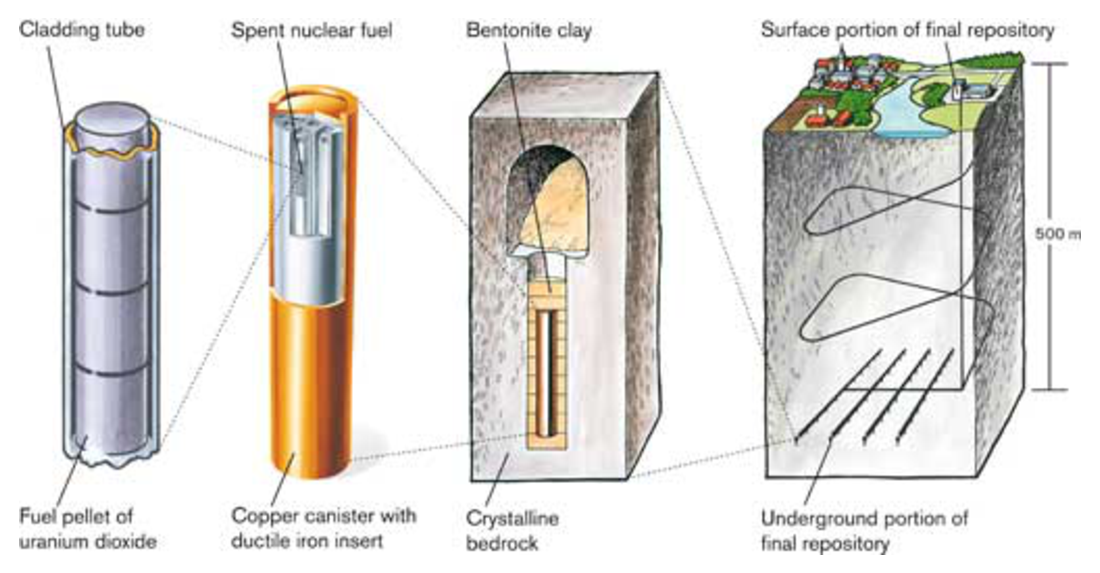
\includegraphics[width=0.7\textwidth]{./images/skb_components.eps}
  \end{center}
  \caption{Geologic disposal systems typically employ engineered barrier 
    systems as well as natural barrier systems. This is a Swedish concept in 
    granite \cite{ab_long-term_2006}.}
  \label{fig:skb_components}
\end{figure}

}
\end{frame}

%%----------------------------------------%%
\begin{frame}[ctb!]
  \frametitle{Engineered Barriers : Waste Forms}
\footnotesize{
  The first line of defense is the waste form.
  \begin{figure}[htbp!]
  \begin{center}
    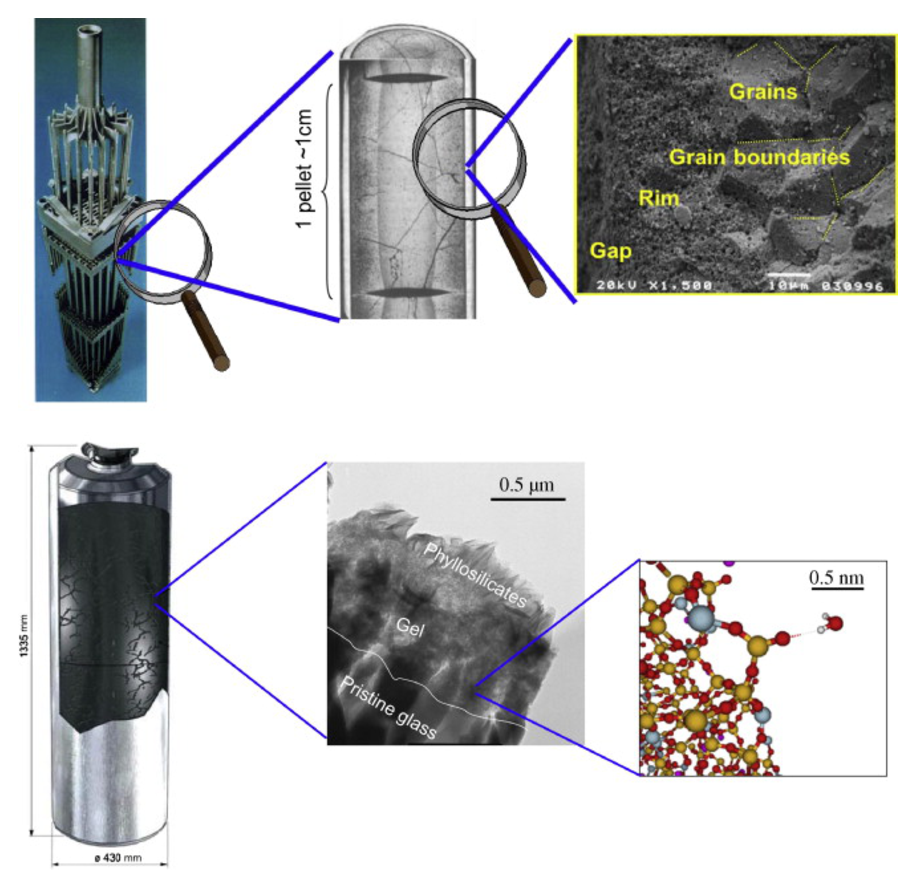
\includegraphics[width=0.5\textwidth]{./images/waste_forms_poinssot.eps}
  \end{center}
  \caption{A comparison of uranium oxide and borosilicate glass waste forms 
  \cite{poinssot_long-term_2012}.}
  \label{fig:waste_forms_poinssot}
\end{figure}

}
\end{frame}

%%----------------------------------------%%
\begin{frame}[ctb!]
  \frametitle{Engineered Barriers : Waste Packages}
\footnotesize{
  \begin{figure}[htbp!]
  \begin{center}
    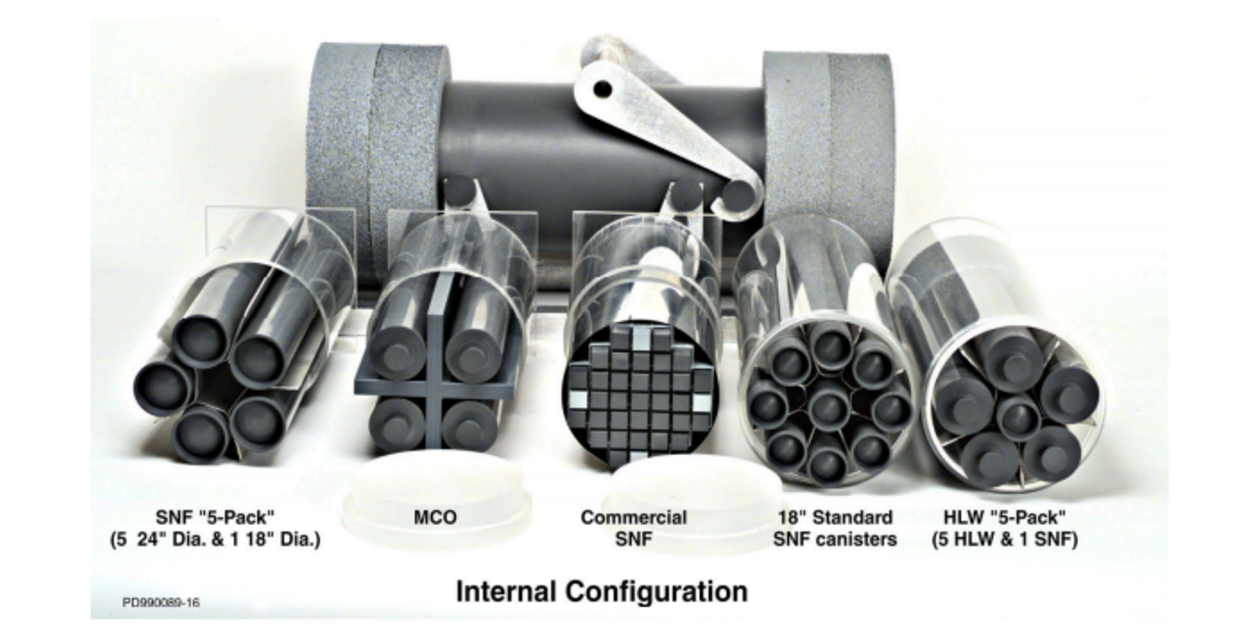
\includegraphics[width=0.7\textwidth]{./images/packages_ineel.eps}
  \end{center}
  \caption{Conceptual mockup of waste packages around waste forms 
    \cite{bridges_standardized_2001}.}
  \label{fig:packages}
\end{figure}

}
\end{frame}

%%----------------------------------------%%
\begin{frame}[ctb!]
  \frametitle{Engineered Barriers : Disposal Cask}
\footnotesize{
  \begin{figure}[htbp!]
  \begin{center}
    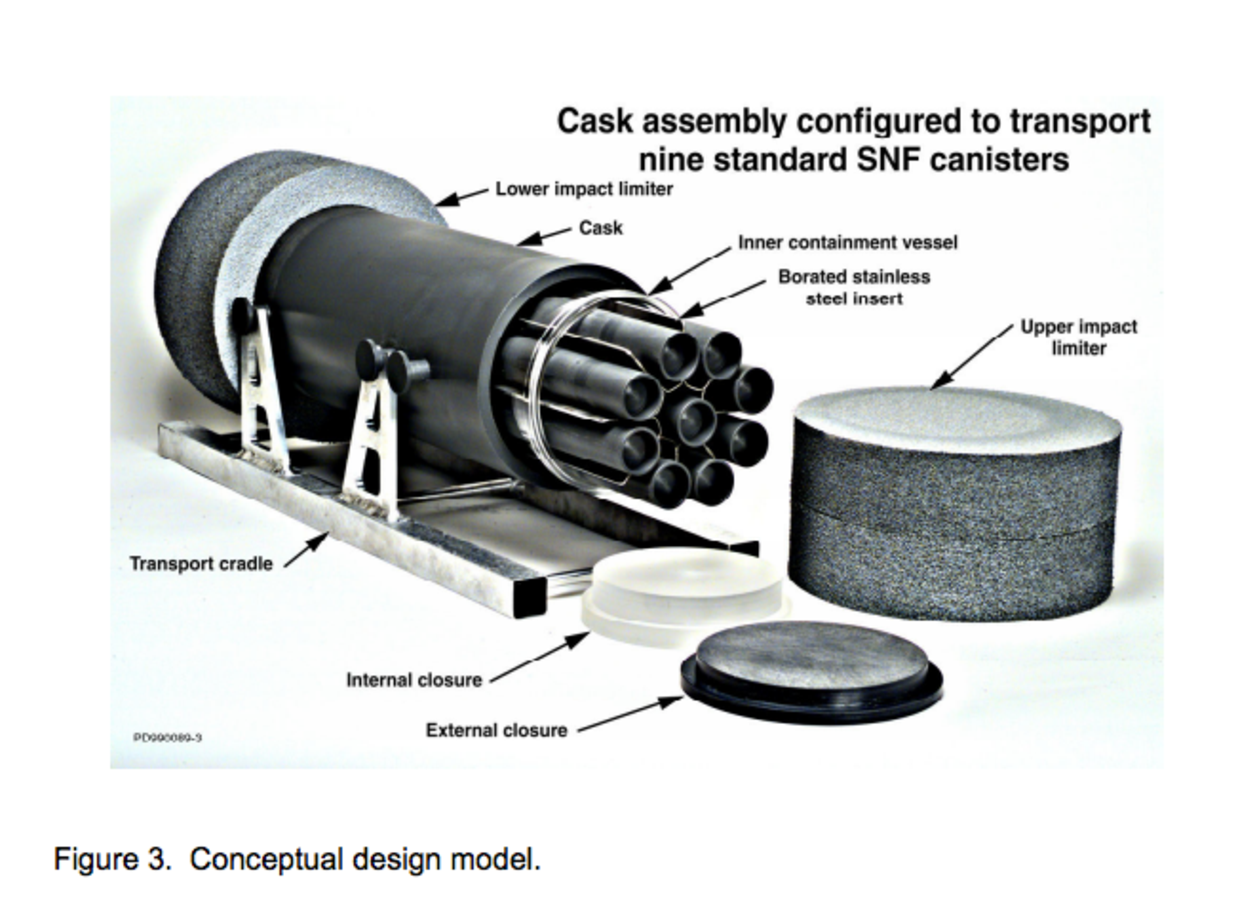
\includegraphics[width=0.7\textwidth]{./images/cask_ineel.eps}
  \end{center}
  \caption{Conceptual mockup of a transport and disposal cask 
    \cite{bridges_standardized_2001}.}
  \label{fig:packages}
\end{figure}

}
\end{frame}

%%----------------------------------------%%
\begin{frame}[ctb!]
  \frametitle{Engineered Barriers : Tunnel}
\footnotesize{
  \begin{figure}[htbp!]
  \begin{center}
    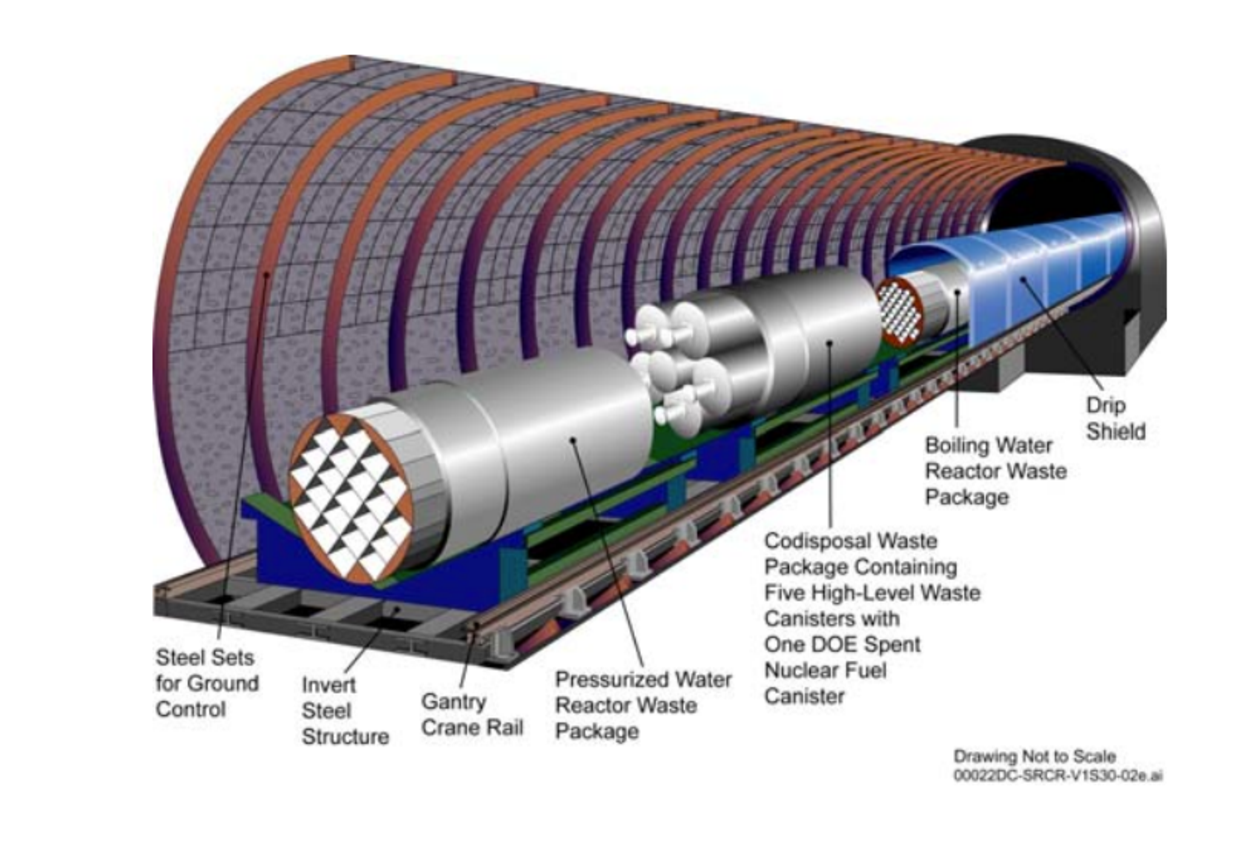
\includegraphics[height=0.7\textwidth]{./images/yucca_tunnel.eps}
  \end{center}
  \caption{The current U.S. geologic disposal concept \cite{peters_whats_2013}.}
  \label{fig:yucca_tunnel}
\end{figure}

}
\end{frame}

%%----------------------------------------%%
\begin{frame}[ctb!]
  \frametitle{Natural Barrier : Geology}
\footnotesize{
  \begin{figure}[htbp!]
  \begin{center}
    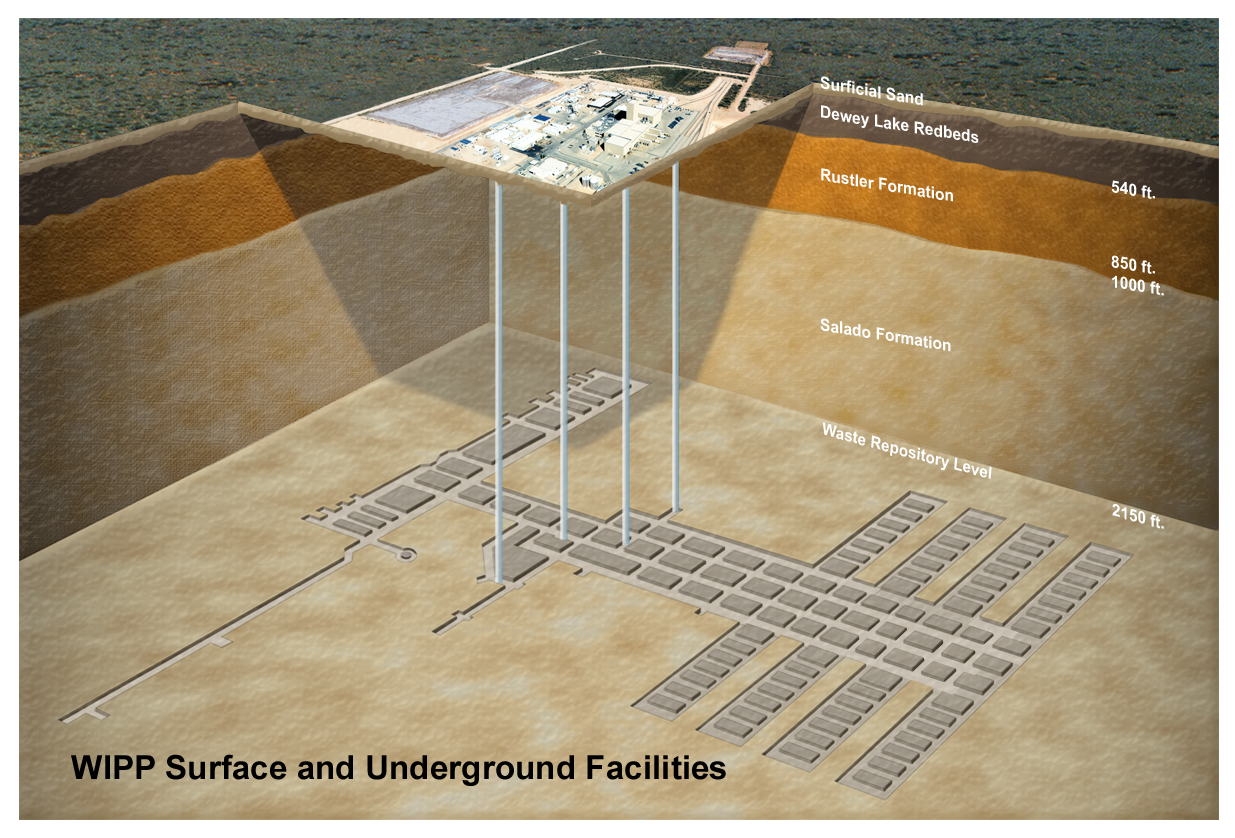
\includegraphics[width=0.7\textwidth]{./images/wipp_stratigraph.eps}
  \end{center}
  \caption{The Waste Isolation Pilot Plant has many geologic layers above the 
    salt bed \cite{doe_wipp_2013}.}
  \label{fig:wipp}
\end{figure}

}
\end{frame}

\begin{frame}
  \frametitle{Repository Layouts}

  \begin{minipage}{0.49\textwidth}
    \begin{figure}[h!]
      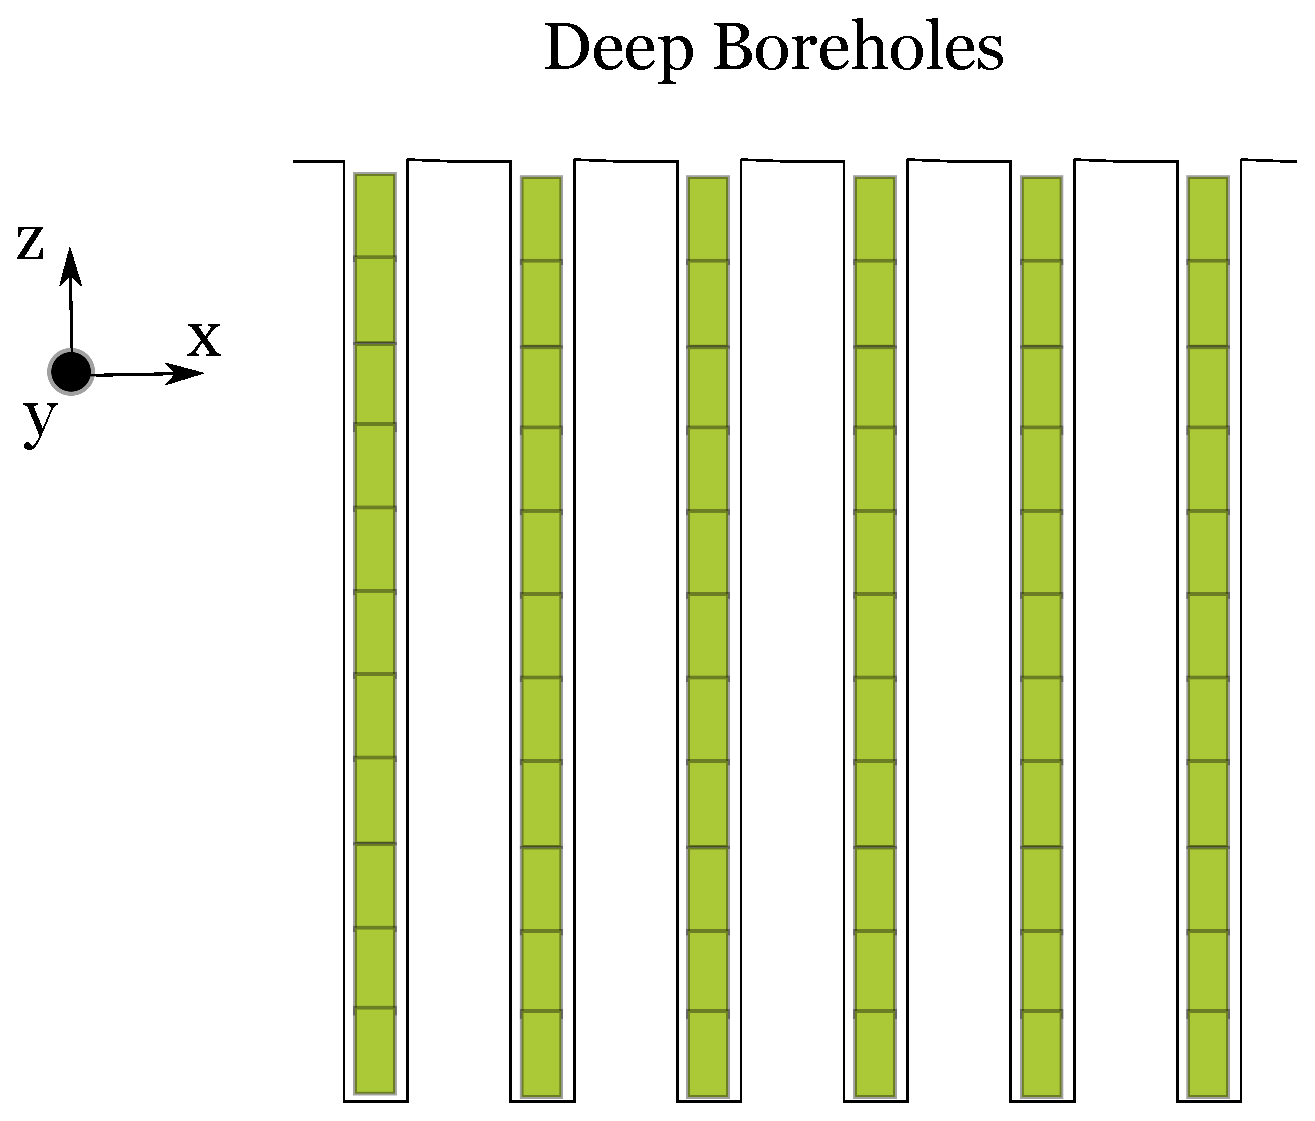
\includegraphics[width=0.75\textwidth]{./images/boreholes.eps}
    \end{figure}
    \begin{figure}[h!]
      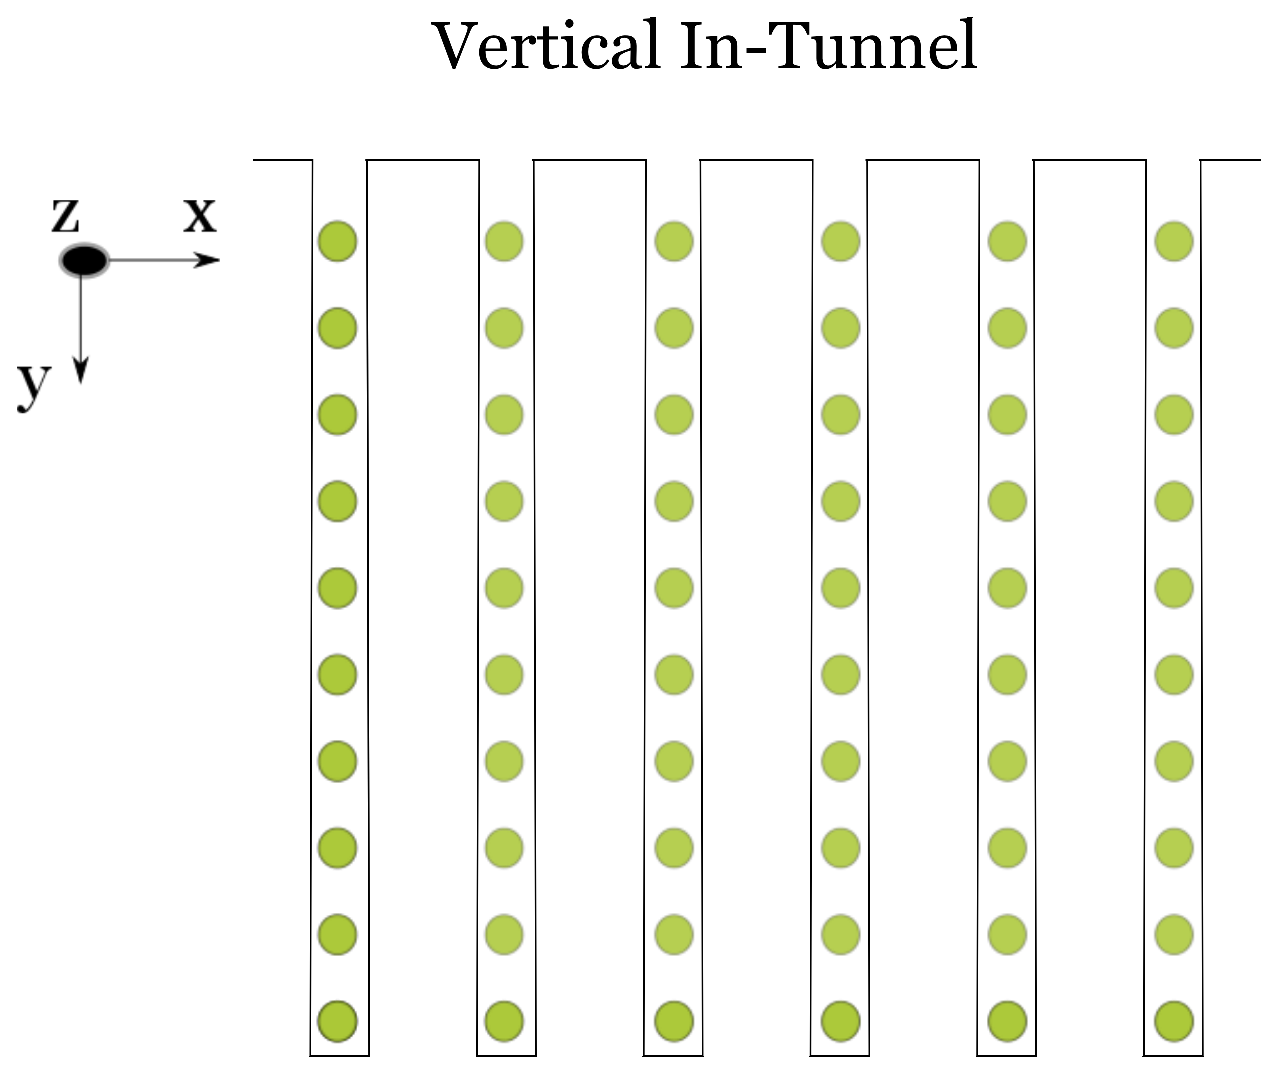
\includegraphics[width=0.75\textwidth]{./images/vertical.eps}
    \end{figure}
  \end{minipage}
  \hspace{0.01cm}
  \begin{minipage}{0.49\textwidth}
    \begin{figure}[h!]
      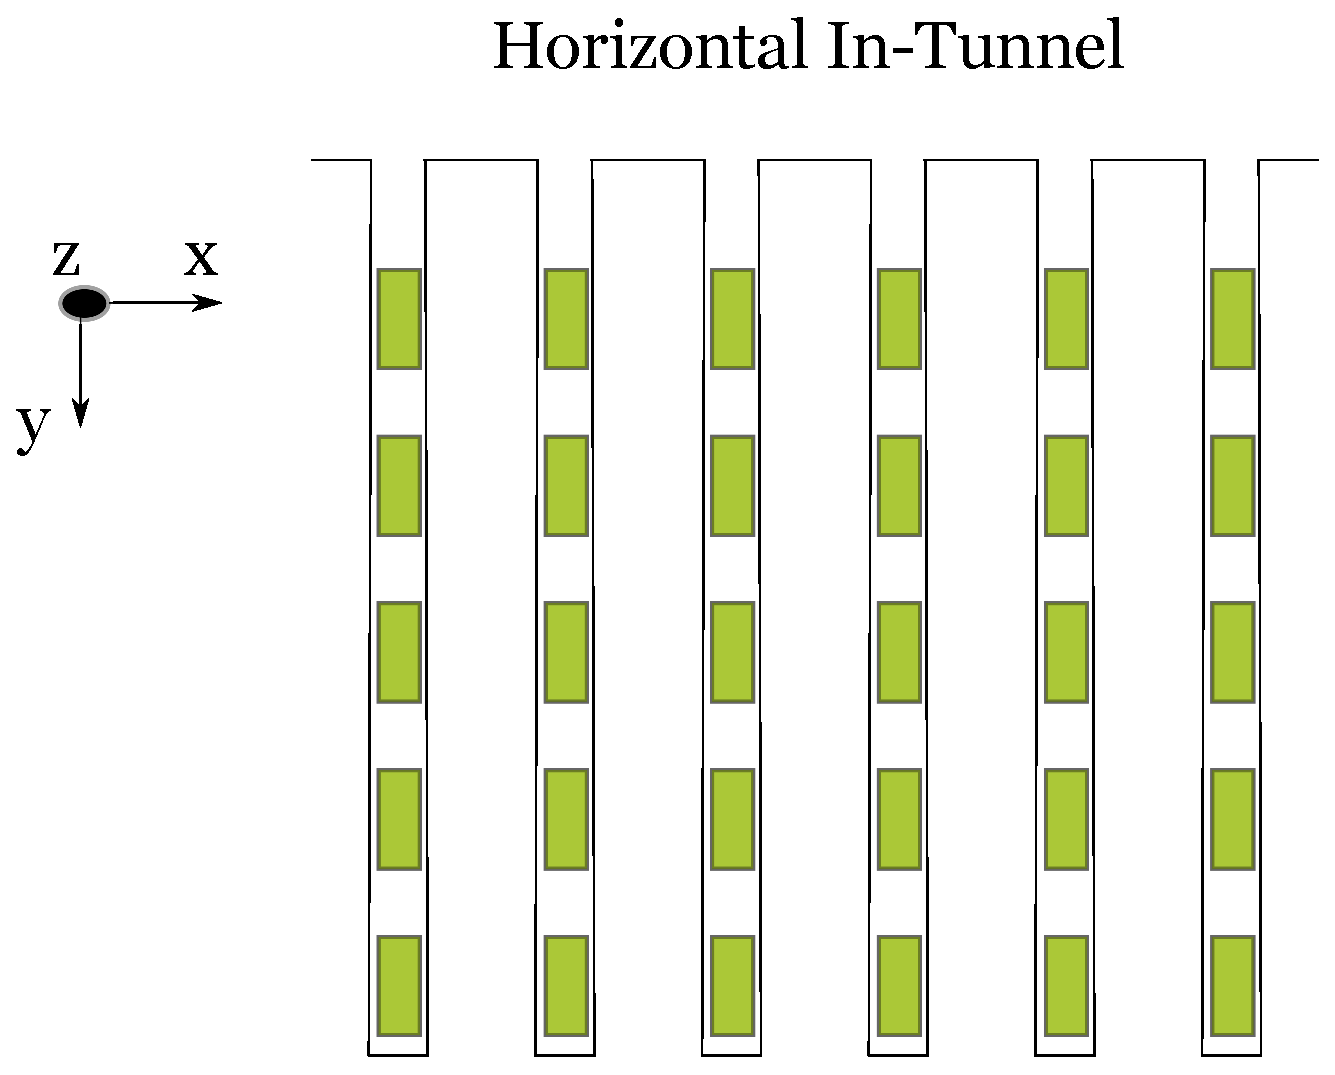
\includegraphics[width=0.8\textwidth]{./images/horizontal.eps}
    \end{figure}
    \begin{figure}[h!]
      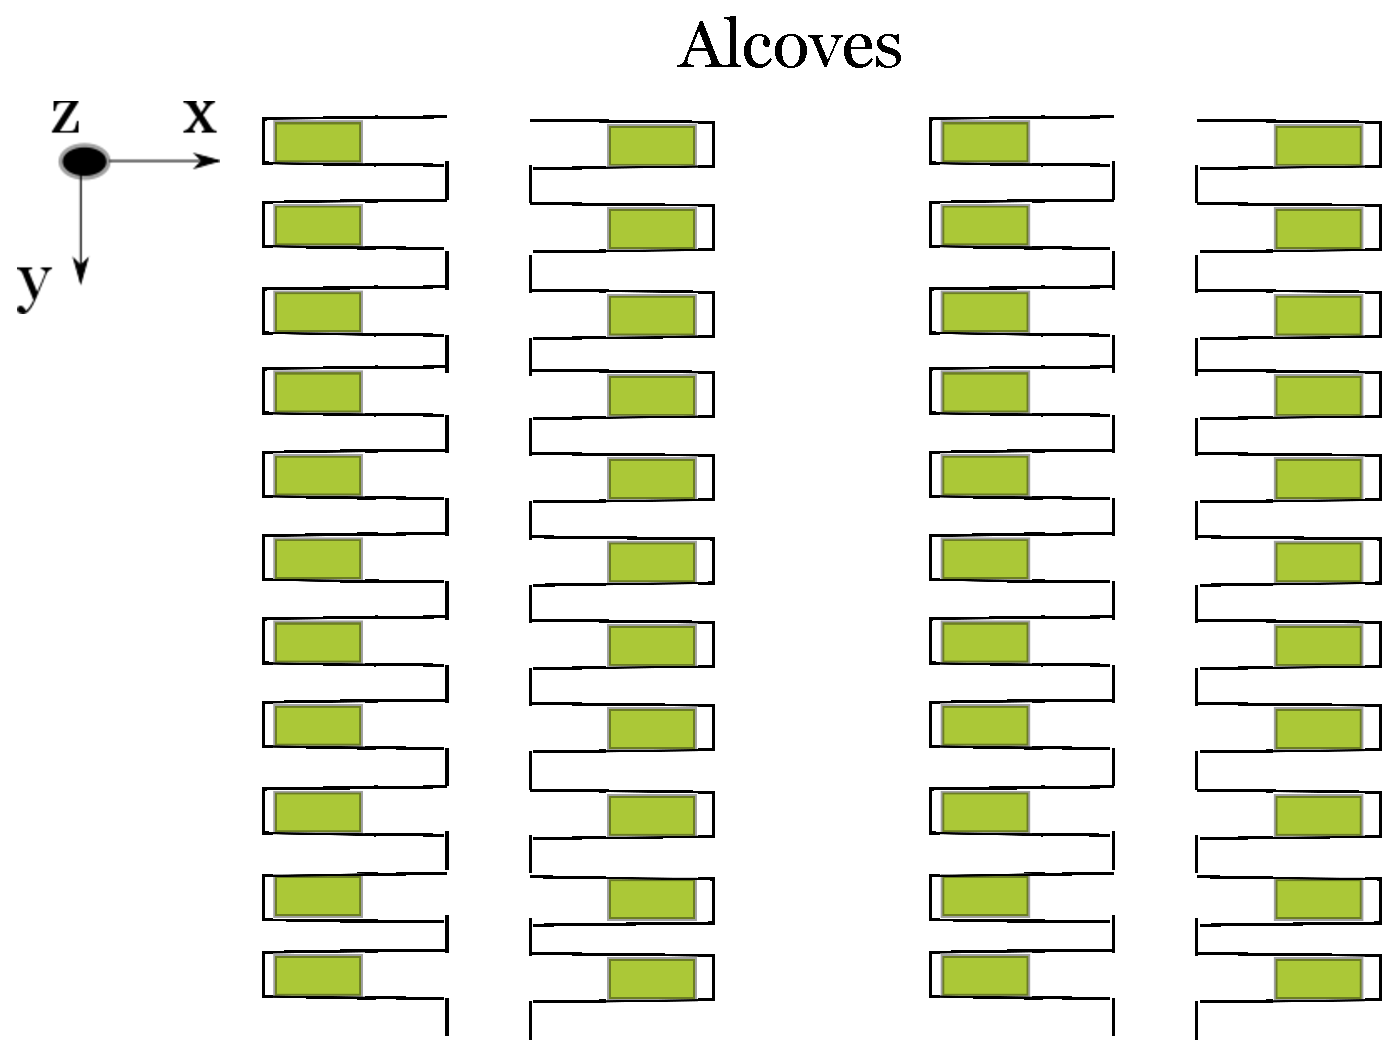
\includegraphics[width=0.8\textwidth]{./images/alcoves.eps}
    \end{figure}
  \end{minipage}

\end{frame}



\begin{frame}[ctb!]
  \frametitle{Tuff (Yucca) Disposal Environments}
  \footnotesize{
    \begin{figure}[htbp!]
  \begin{center}
    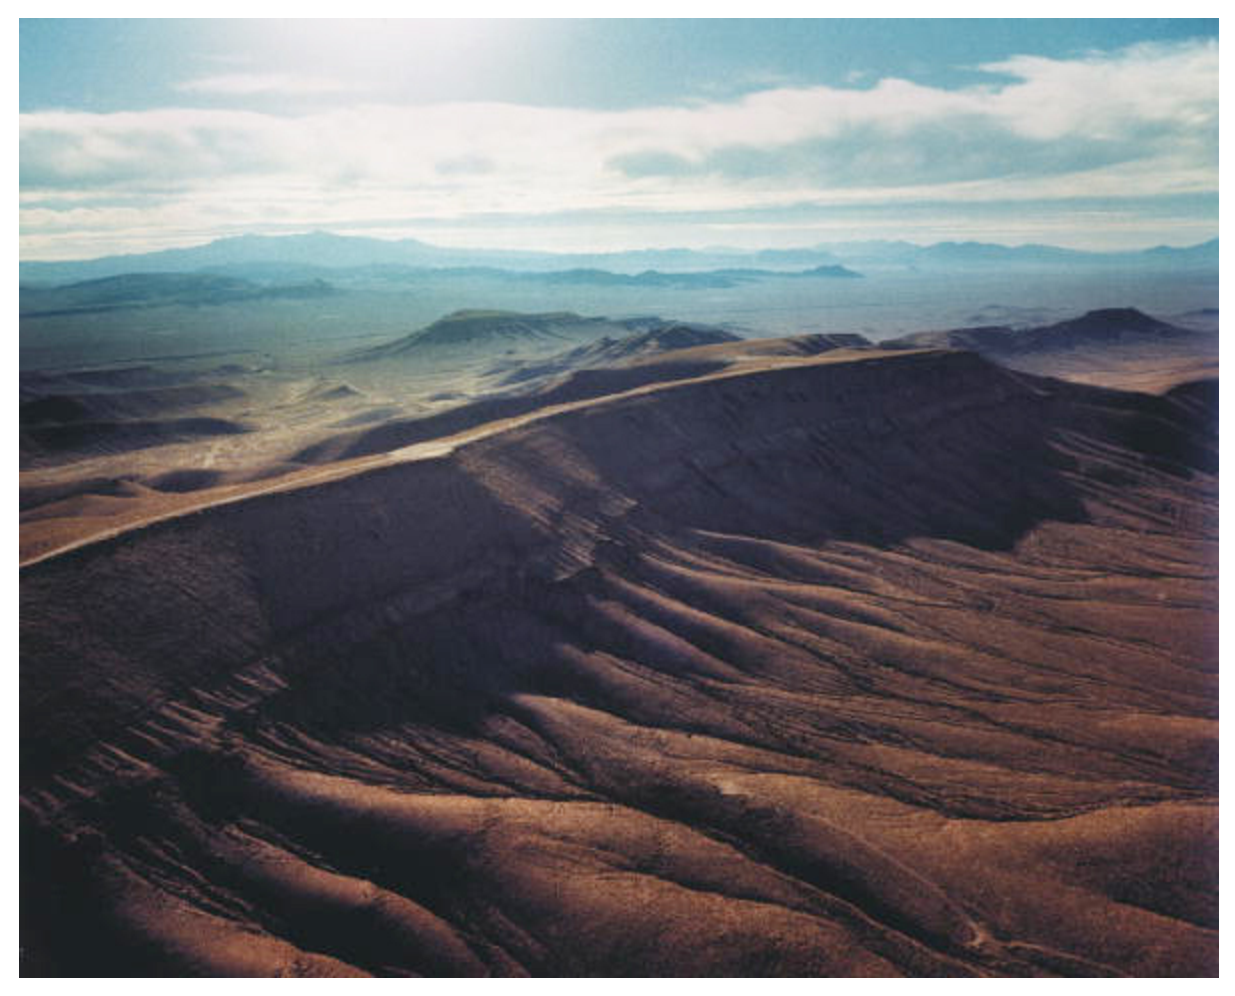
\includegraphics[width=0.5\textwidth]{./images/yucca_site.eps}
  \end{center}
  \caption{Yucca Mountain is in southern Nevada \cite{omb_yucca_2006}.}
  \label{fig:yucca_site}
\end{figure}

  }
\end{frame}

\begin{frame}[ctb!]
  \frametitle{Alternative Disposal Geology Options}
   \begin{minipage}{0.44\textwidth}
     \begin{figure}[h!]
         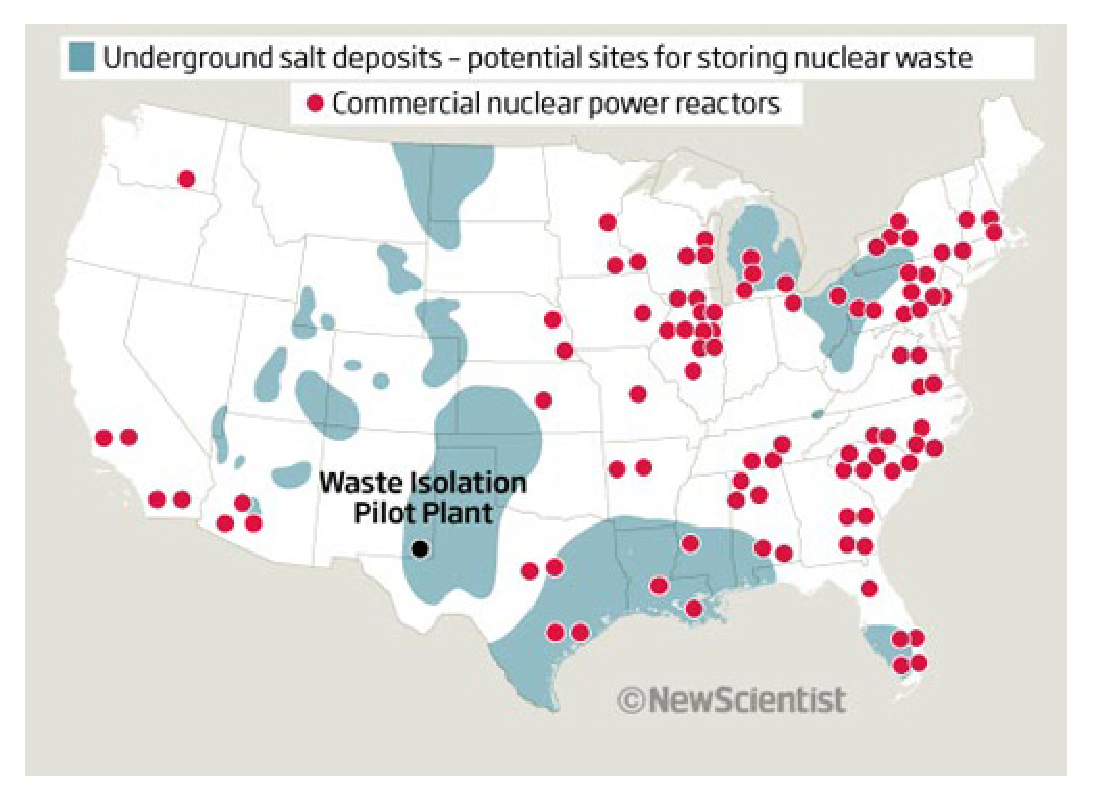
\includegraphics[width=0.8\textwidth]{./images/saltNewScientist.eps}
         \caption{U.S. Salt Deposits, ref. \cite{newscientist_where_2011}.}
     \end{figure}
     \begin{figure}[h!]
         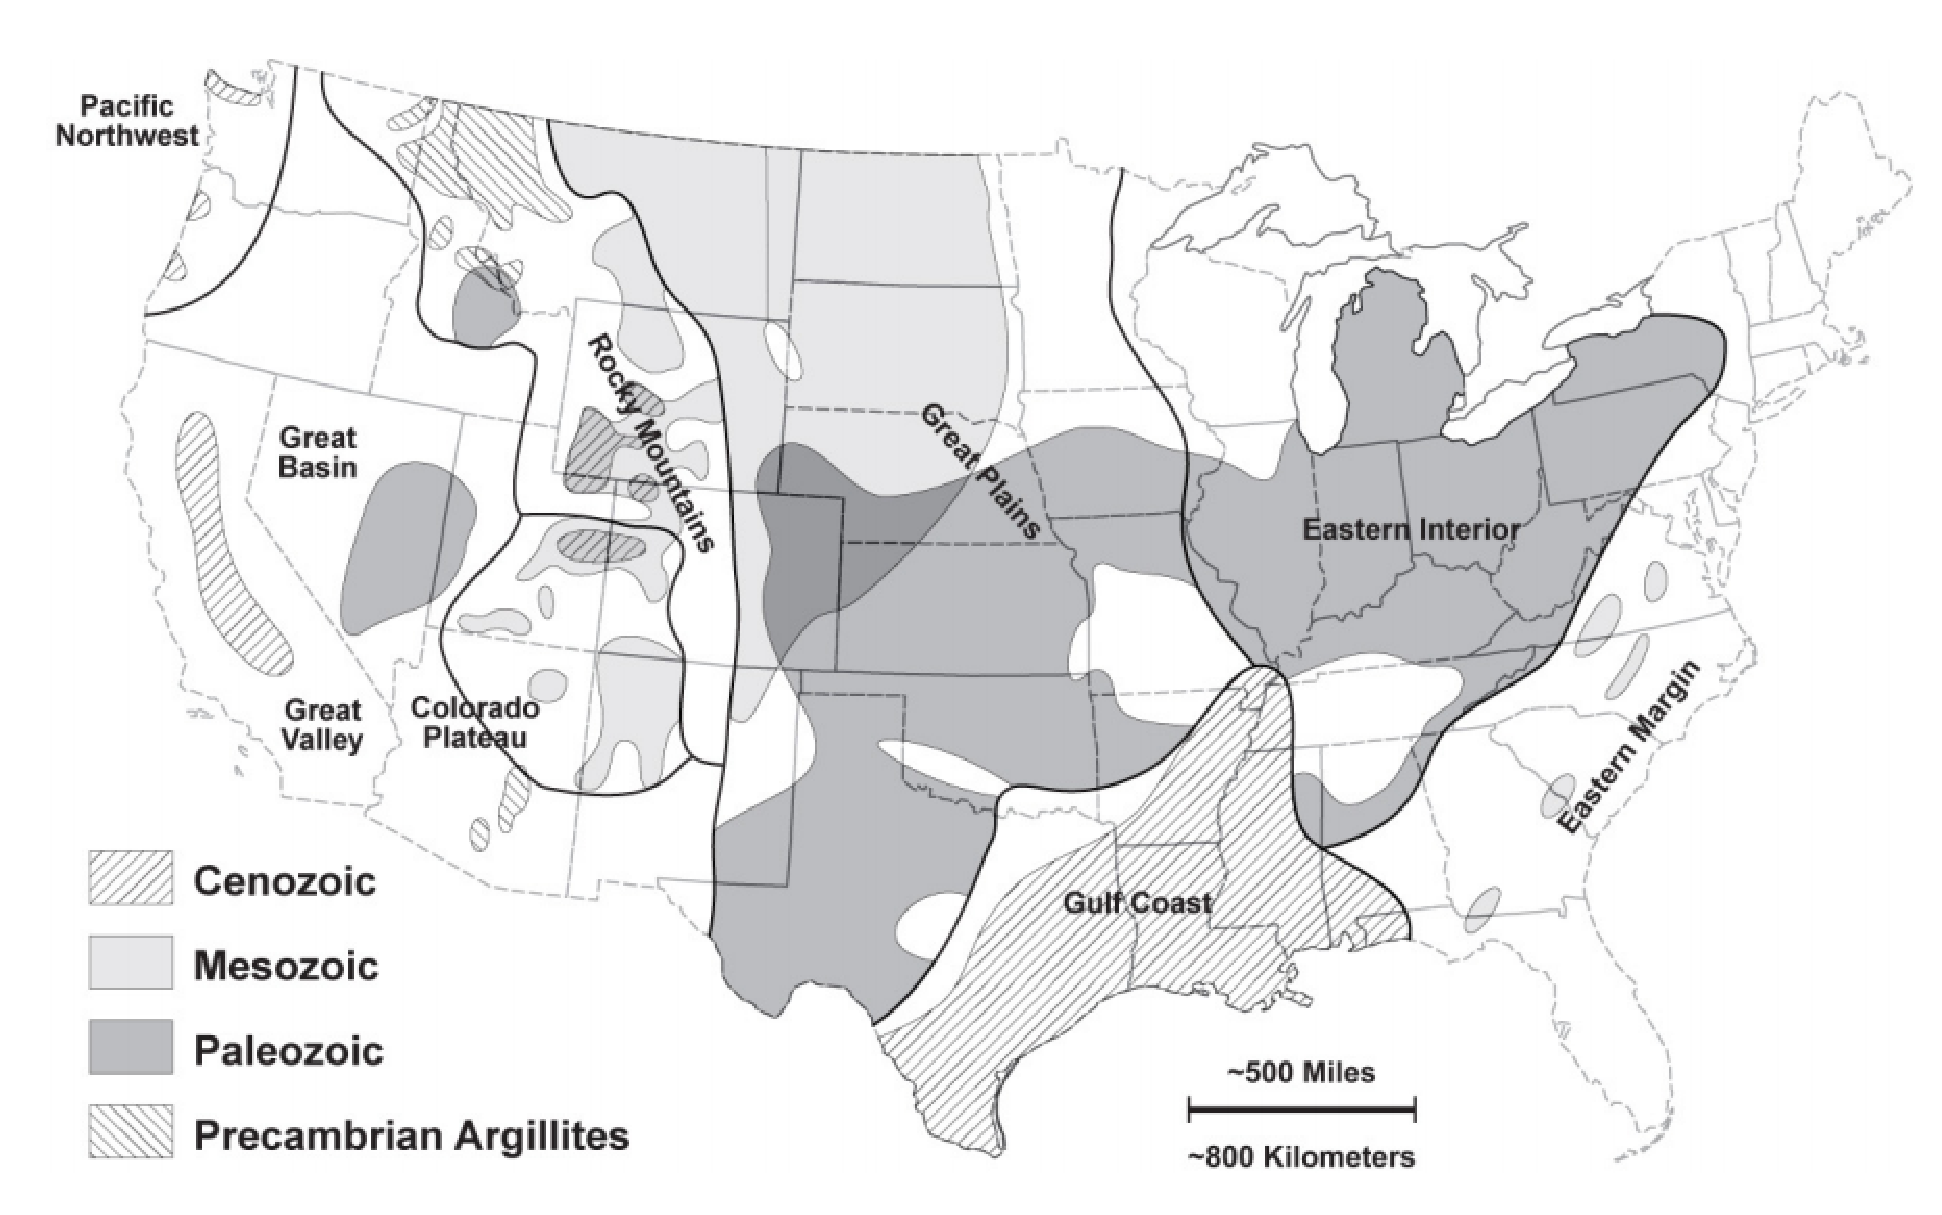
\includegraphics[width=0.8\textwidth]{./images/clayGonzales.eps}
         \caption{U.S. Clay Deposits, ref. \cite{gonzales_shales_1985}.}
     \end{figure}
   \end{minipage}
   \hspace{0.01cm}
   \begin{minipage}{0.44\textwidth}
     \begin{figure}[h!]
         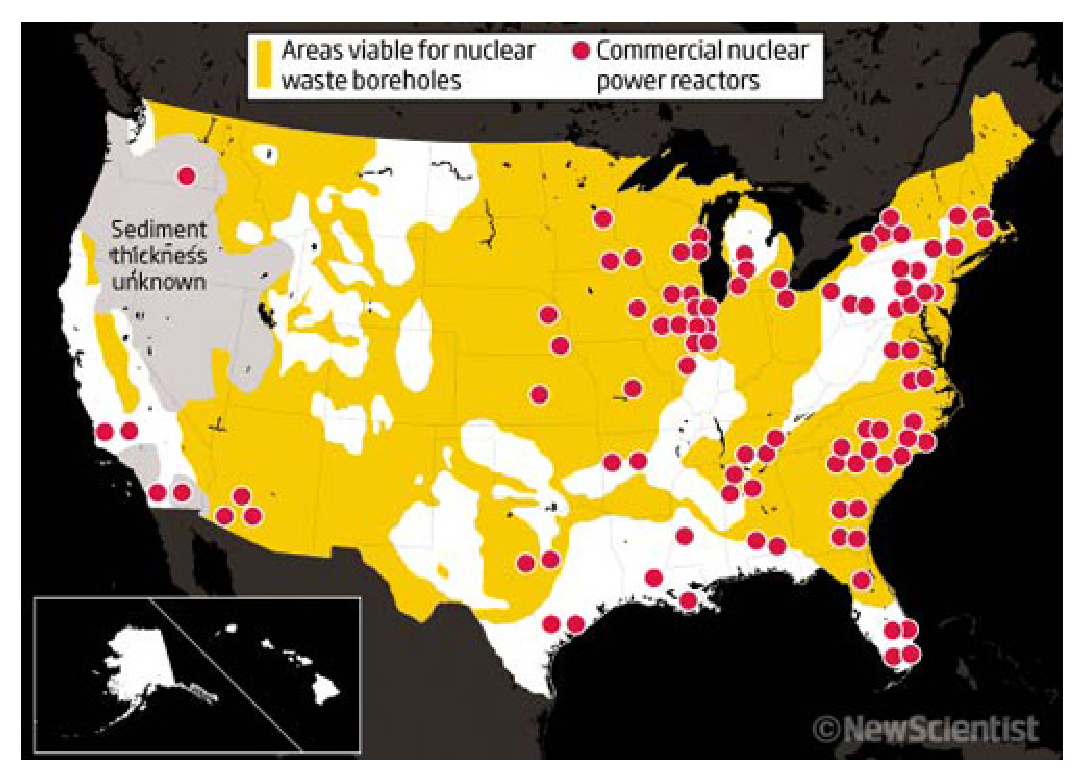
\includegraphics[width=0.8\textwidth]{./images/boreholeNewScientist.eps}
         \caption{U.S. Crystalline Basement, ref.  \cite{newscientist_where_2011}.}
     \end{figure}
     \begin{figure}[h!]
         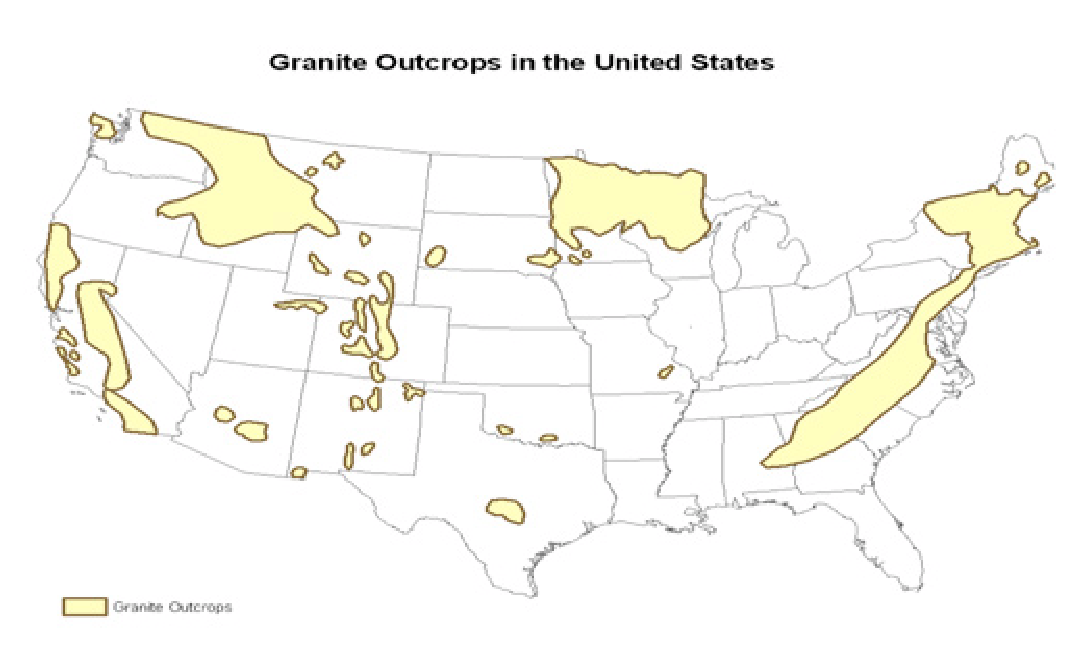
\includegraphics[width=0.8\textwidth]{./images/graniteBush.eps}
         \caption{U.S. Granite Beds, ref. \cite{bush_economic_1976}.}
     \end{figure}
   \end{minipage}
\end{frame}

\begin{frame}[ctb!]
  \frametitle{Clay Disposal Environments}
  \footnotesize{

  \begin{figure}[h!]
    \begin{center}
      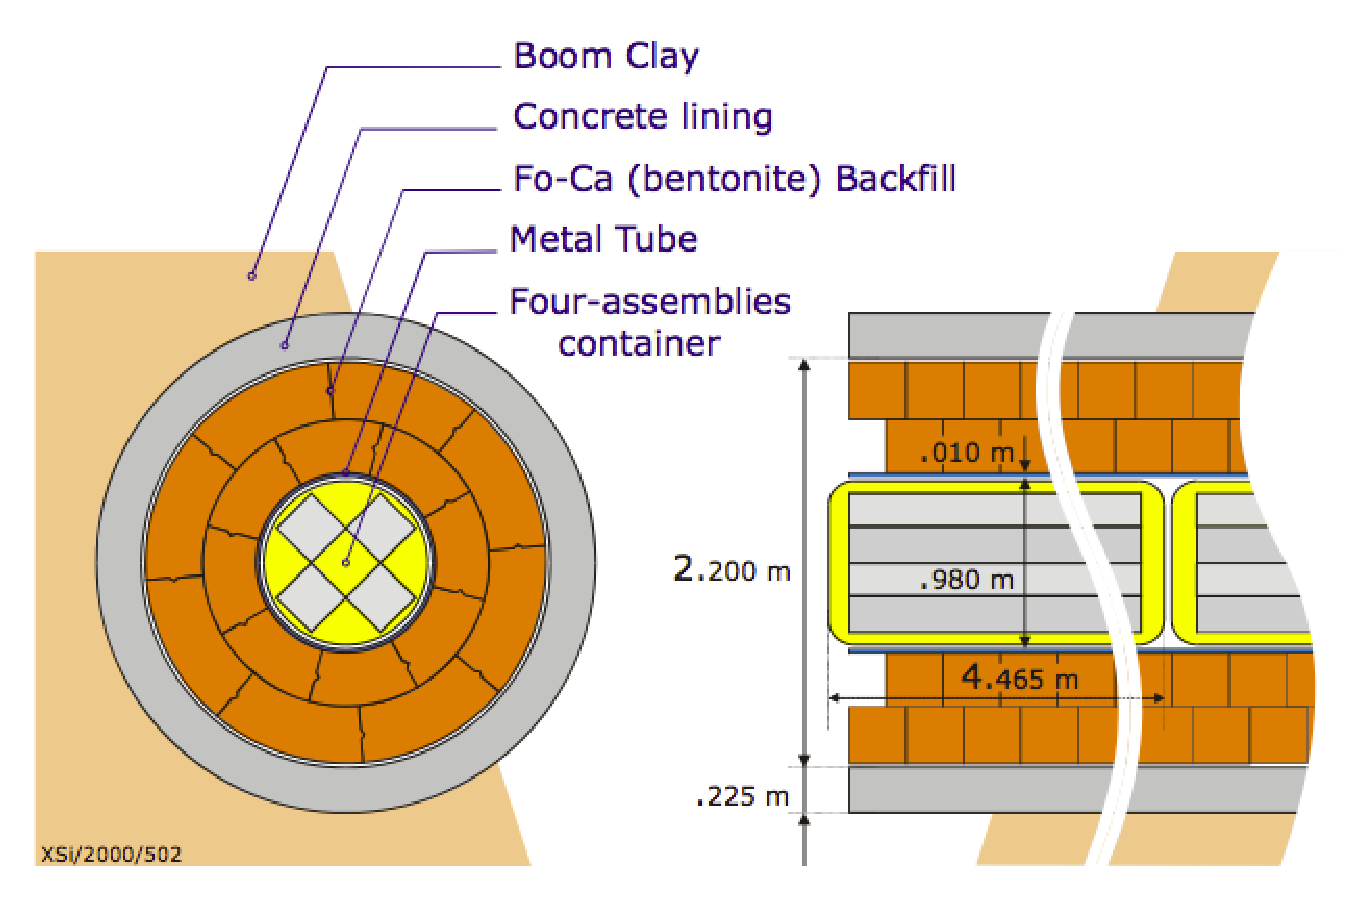
\includegraphics[height=.7\textheight]{./images/belgianClayRedImp.eps}
    \end{center}
    \caption{Belgian reference concept in Boom Clay 
    \cite{von_lensa_red-impact_2008}.}
    \label{fig:belgianClayRedImp}
  \end{figure}

}
\end{frame}

\begin{frame}[ctb!]
  \frametitle{Granite Disposal Environments}
  \footnotesize{

  \begin{figure}[h!]
    \begin{center}
      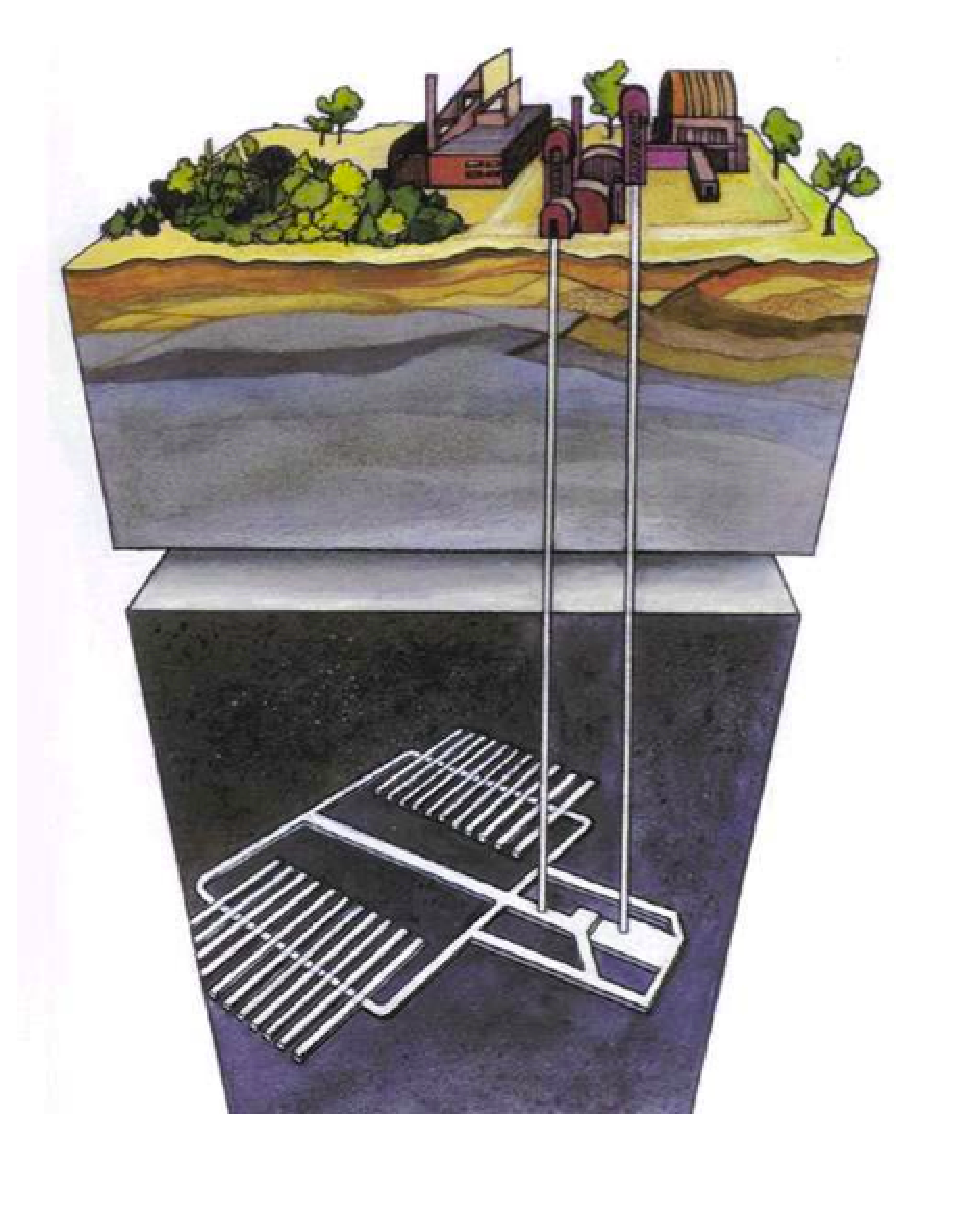
\includegraphics[height=.7\textheight]{./images/czechGraniteRedImp.eps}
    \end{center}
    \caption{Czech reference concept in Granite 
    \cite{von_lensa_red-impact_2008}.}
    \label{fig:czechGraniteRedImp}
  \end{figure}
}
\end{frame}

\begin{frame}[ctb!]
  \frametitle{Salt Disposal Environments}
  \footnotesize{

  \begin{figure}[h!]
    \begin{center}
      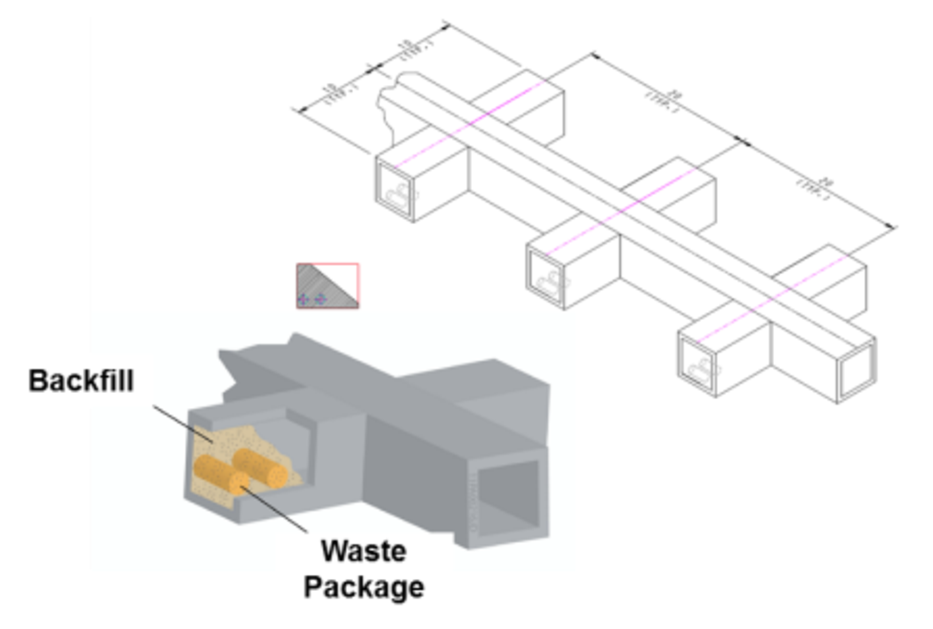
\includegraphics[height=.7\textheight]{./images/carter_salt_layout.eps}
    \end{center}
    \caption{DOE-NE Used Fuel Disposition Campaign  concept in 
    Salt \cite{hardin_generic_2011}.}
    \label{fig:salt_layout}
  \end{figure}
}
\end{frame}
\begin{frame}[ctb!]
  \frametitle{Salt Disposal Environments}
  \footnotesize{

  \begin{figure}[h!]
    \begin{center}
      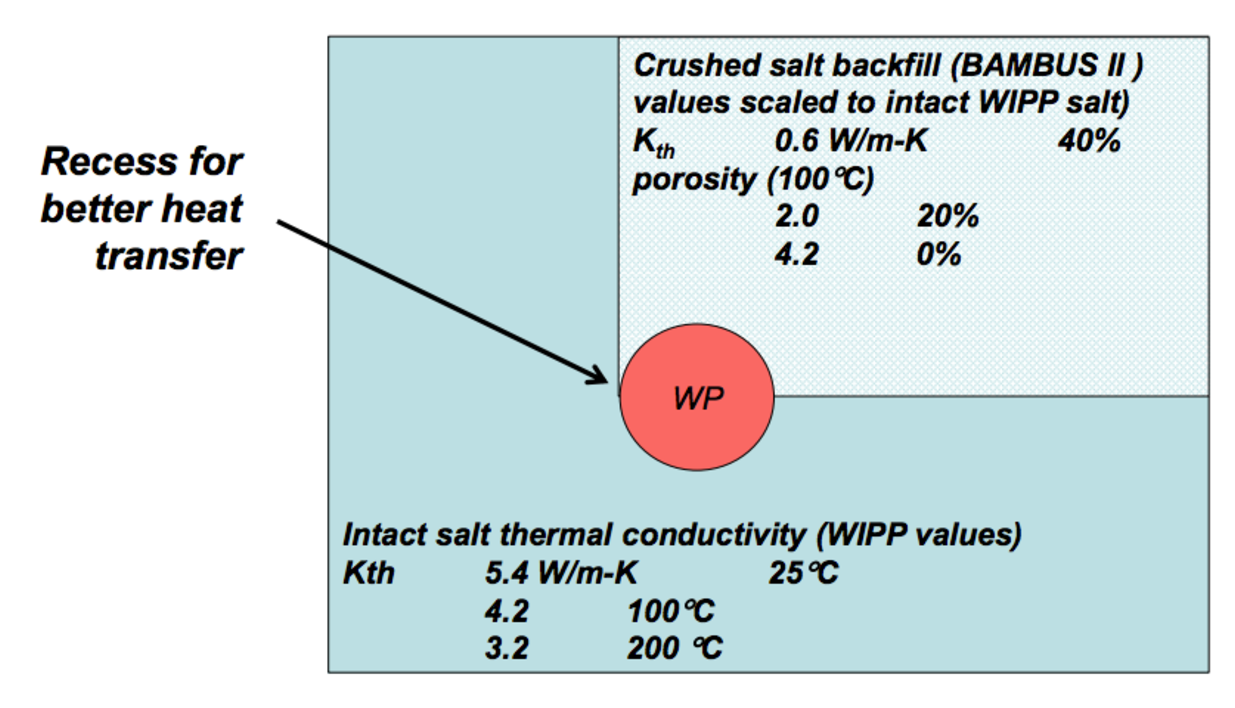
\includegraphics[height=.7\textheight]{./images/hardin_salt_layout.eps}
    \end{center}
    \caption{DOE-NE Used Fuel Disposition Campaign  concept in 
    Salt \cite{hardin_generic_2011}.}
    \label{fig:hardin_salt_layout}
  \end{figure}
}
\end{frame}

\begin{frame}[ctb!]
  \frametitle{Deep Borehole Disposal Environment}
  \footnotesize{

  \begin{figure}[h!]
    \begin{center}
      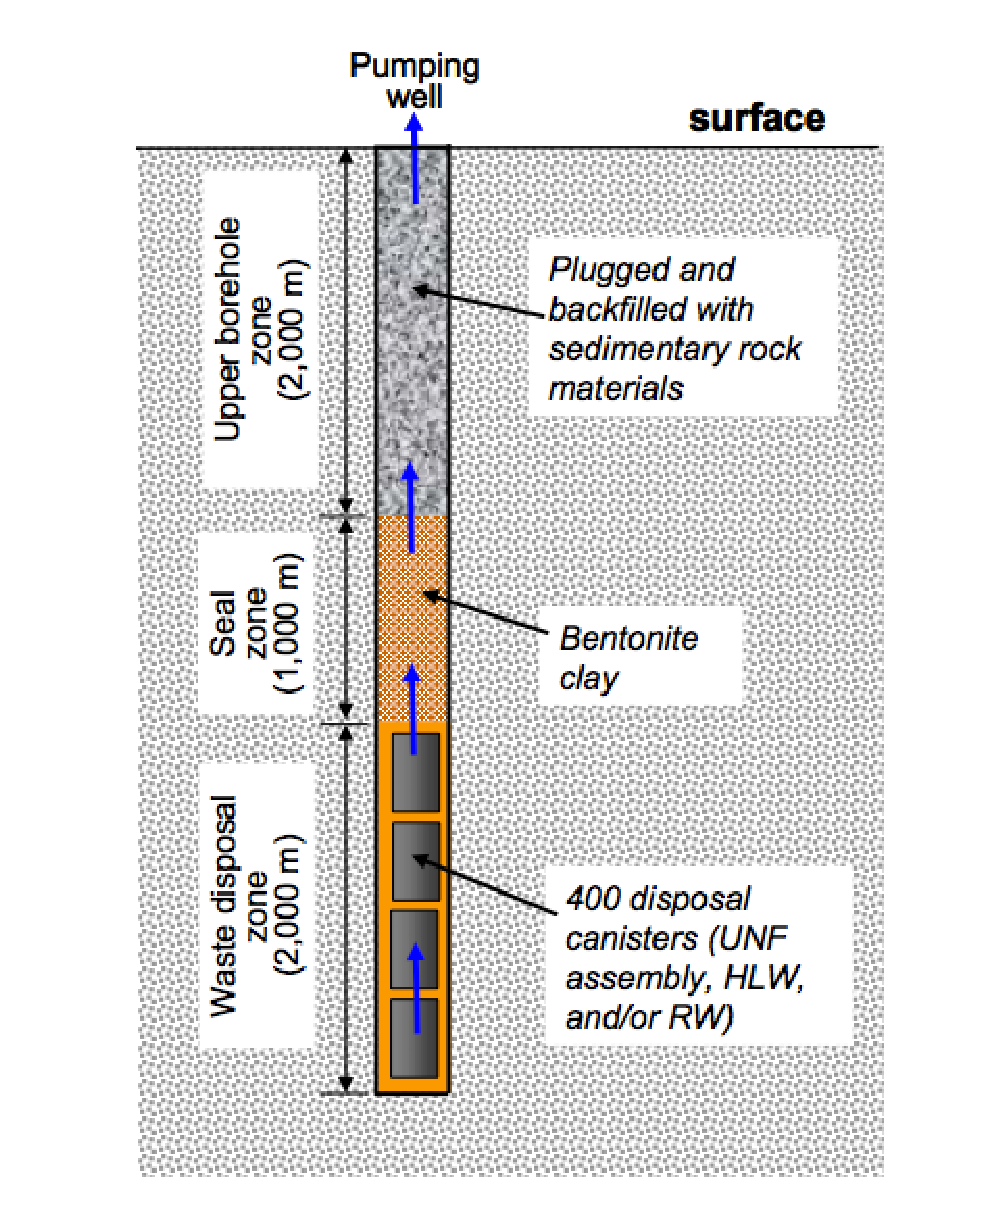
\includegraphics[height=.7\textheight]{./images/boreholeGPAM.eps}
    \end{center}
    \caption{DOE-NE Used Fuel Disposition Campaign Deep Borehole concept 
    \cite{hardin_generic_2011}.}
    \label{fig:boreholeGPAM}
  \end{figure}
}
\end{frame}


\subsection{Fuel Cycle Simulator Capabilities}

\section{Geologic Repository Performance}
\subsection{Metrics}
\include{performance_metrics}
\subsection{Thermal Loading}
\include{performance_thermal}
\subsection{Radionuclide Transport and Release}
\include{performance_release}

\section{Modeling Paradigm}
\subsection{Cyclus Modeling Paradigm}
\subsection{Cyder Modeling Paradigm}


\section{Abstracted Models}
\subsection{Thermal Transport in Cyder}
\subsection{Supporting Thermal Response Dataset}
To support this calculation in \Cyder , a reference data set of temperature change 
curves was calculated. Repeated runs of a detailed analytic model over the range of values in Table 
\ref{tab:thermal_cases} determined \gls{STC} values over a range of thermal 
heat limit radii, $r_{lim}$, thermal diffusivity values, $\alpha_{th}$,
thermal conductivity values, $K_{th}$ and waste package spacings, $S$. Linear 
interpolation across the discrete parameter space provides a simple thermal 
reference dataset for use in \Cyder .

\begin{table}[ht!]
\centering
\footnotesize{
\begin{tabular}{|l|l|l|r|}
\multicolumn{4}{c}{\textbf{Thermal Cases}}\\
\hline
\textbf{Parameter} & \textbf{Symbol} & \textbf{Units} & \textbf{Value Range} \\
\hline
Diffusivity & $\alpha_{th}$ & $[m^2\cdot s^{-1}]$ & $1.0\times10^{-7}$\\
 & & & $2.0\times10^{-7}$\\
 & & & $3.0\times10^{-7}$\\
 & & & $4.0\times10^{-7}$\\
 & & & $5.0\times10^{-7}$\\
 & & & $6.0\times10^{-7}$\\
 & & & $7.0\times10^{-7}$\\
 & & & $8.0\times10^{-7}$\\
 & & & $9.0\times10^{-7}$\\
 & & & $1.0\times10^{-6}$\\
 & & & $2.0\times10^{-6}$\\
 & & & $3.0\times10^{-6}$\\
\hline
Conductivity & $K_{th}$     & $[W\cdot m^{-1} \cdot K^{-1}]$  & $0.1, 0.5, 1, 1.5, 2, 2.5, 3, 3.5, 4, 4.5 $ \\
\hline
Spacing & $S$ & $[m]$ & 2, 5, 10, 15, 20, 25, 50 \\
\hline
Radius & $r_{lim}$ & $[m]$ & 0.1, 0.25, 0.5, 1, 2, 5 \\
\hline
Isotope & $i$ & $[-]$ & $^{241,243}Am,$  \\
        & & & $^{242,243,244,245,246}Cm,$  \\
        & & & $^{238,240,241,242}Pu$  \\
        & & & $^{134,135,137}Cs$  \\
        & & & $^{90}Sr$  \\
\hline
\end{tabular}
\caption{A thermal reference dataset of \gls{STC} values as a function of each of these parameters was generated by repeated parameterized runs of the LLNL 
MathCAD model\cite{greenberg_application_2012, greenberg_investigations_2012}.}
\label{tab:thermal_cases}
}
\end{table}



The analytic model used to populate the reference dataset was created at 
\gls{LLNL} for the \gls{UFD} campaign. In this tool, heat limited thermal 
response is calculated analytically for each geology, for many waste package 
loading densities, and for many fuel cycle options \cite{hardin_generic_2011, 
greenberg_investigations_2012, greenberg_application_2012}. It employs an 
analytic model from Carslaw and Jaeger and is implemented in MathCAD 
\cite{carslaw_conduction_1959, ptc_mathcad_2010}.  The integral solver in the 
MathCAD toolset is the primary calculation engine for the analytic MathCAD 
thermal model, which relies on superposition of point, finite-line, and line 
source integral solutions.  

%The transient state of the temperature at the calculation radius is found with a convolution of the transient far field solution with the steady state near field solution.  The process is then iterated with a one year resolution in order to arrive at a temperature evolution over the lifetime of the repository. 
%
%In a two dimensional grid of waste packages, the central package is represented by the finite line solution

Figure \ref{fig:CmScaling} demonstrates the scaling of an STC curve according to 
equation \eqref{STC} to represent the heat from $25.9g$ of initial $^{242}Cm$ using 
the reference data set. 

\begin{figure}[h!]
\begin{center}
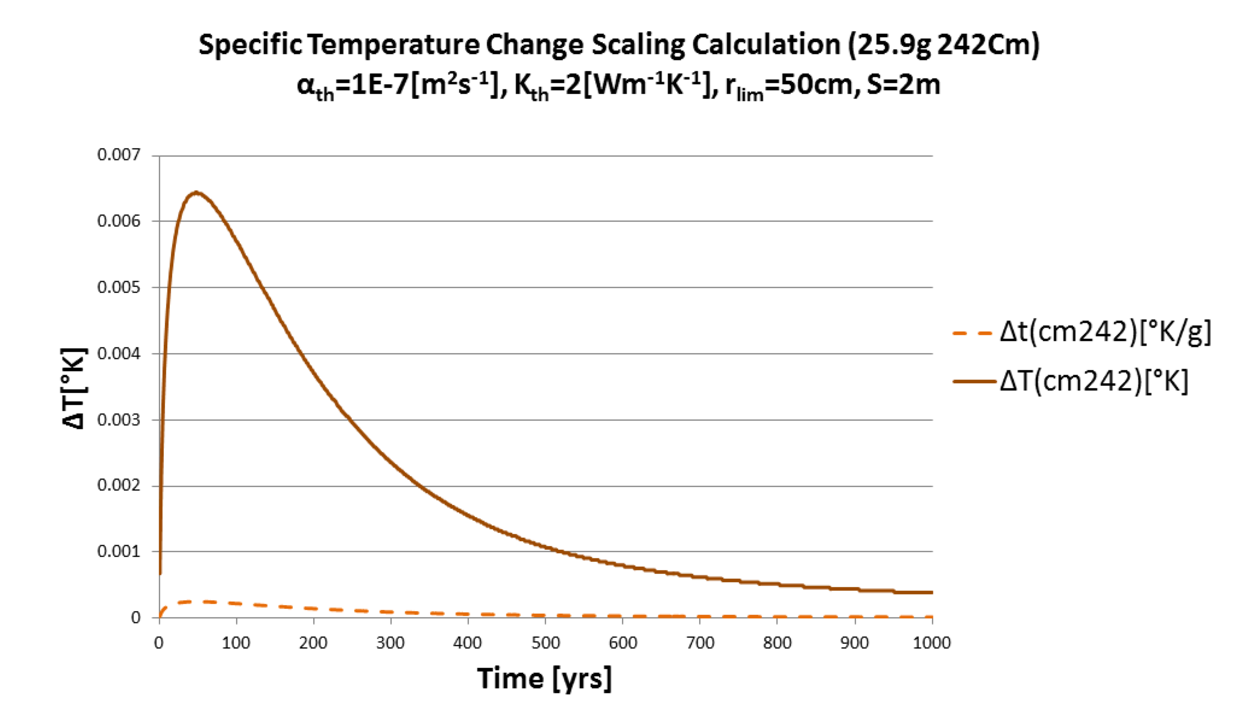
\includegraphics[width=\columnwidth]{./thermal_models/CmScaling.eps}
\end{center}
\caption{As a demonstration of the calculation procedure, the temperature change 
  curve for one initial gram of $^{242}Cm$ and is scaled to represent $25.9g$, 
  approximately the $^{242}Cm$ inventory per MTHM in 51GWd burnup UOX PWR fuel. }
\label{fig:CmScaling}
\end{figure}


The supporting database was limited to some primary heat contributing isotopes 
present in traditional spent nuclear fuel, $H$, 
such that the superposition in equation \eqref{superposition} becomes 

\begin{align}
\Delta T (r_{lim},S,K_{th},\alpha_{th})&\sim \sum_{i\in H} m_i \Delta t_i(r_{lim},S,K_{th},\alpha_{th})
\label{superposition_approx}
\intertext{where}
H &= \mbox{ set of high heat isotopes }[-]\nonumber\\
S &= \mbox{ uniform waste package spacing } [m]\nonumber\\
K_{th} &= \mbox{ thermal conductivity } [W\cdot m^{-1}\cdot K^{-1}]\nonumber\\
\alpha_{th} &= \mbox{ thermal diffusivity } [m^2\cdot s^{-1}]\nonumber\\
\end{align}

The use of this superposition is demonstrated in Figure 
\ref{fig:CmSuperposition}.

\begin{figure}[ht!]
\begin{center}
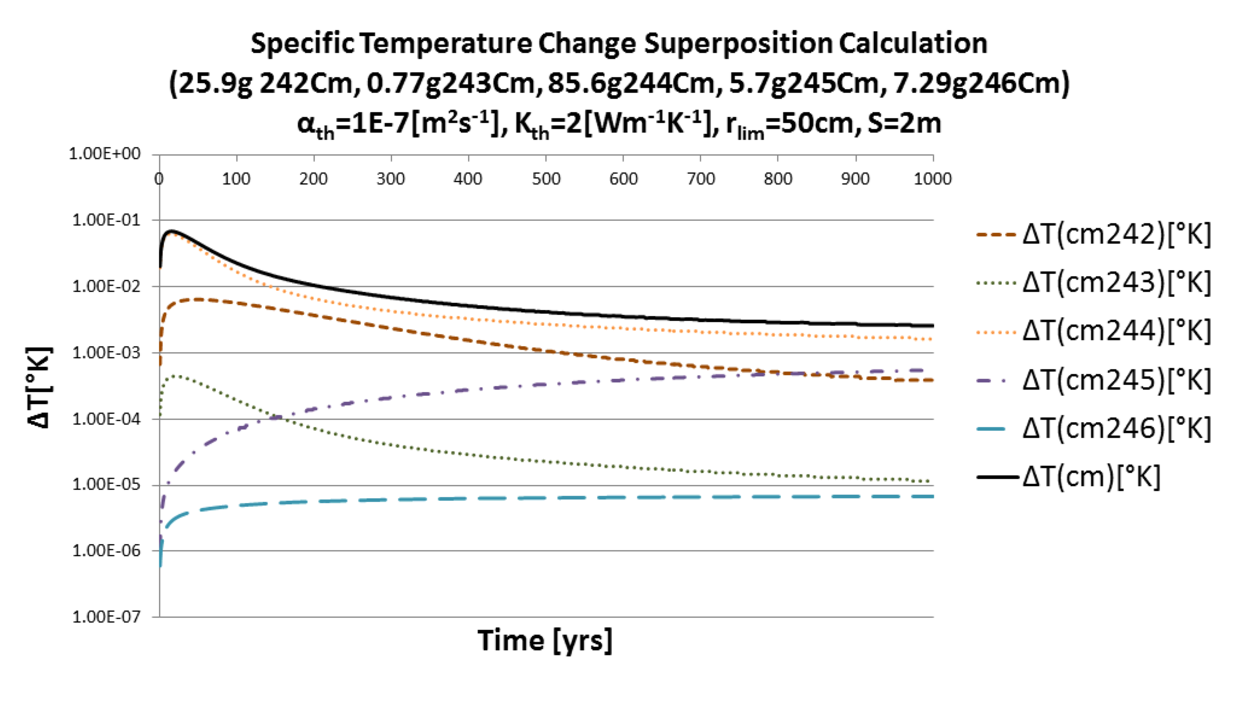
\includegraphics[width=\columnwidth]{./thermal_models/CmSuperposition.eps}
\end{center}
\caption{As a demonstration of the calculation procedure, scaled temperature change 
  curves for five curium isotopes are superimposed to achieve a total temperature 
change (note log scale).}
\label{fig:CmSuperposition}
\end{figure}

%\begin{align}
%  T_{line}(t,x,y,z) &= \frac{1}{8\pi K_{th}} 
%  \bigintsss_0^t\!\frac{q_L(t')}{t-t'}e^{ \frac{-\left(x^2 + z^2\right)}{4\alpha 
%  (t-t')} }\nonumber\\ &\cdot\left[ \erf{\left[ \frac{1}{2} \frac{\left( y + 
%  \frac{L}{2} \right)}{\sqrt{\alpha(t-t')}}  \right]} - \erf{\left[ \frac{1}{2} 
%  \frac{\left( y - \frac{L}{2} \right)}{\sqrt{\alpha(t-t')}}  \right]} 
%  \right]\,\mathrm{dt'},
%  \label{line}
%  \intertext{adjacent packages within the central tunnel are represented by the 
%  point source solution }
%  T_{point}(t,r) &= 
%  \frac{1}{8K_{th}\sqrt{\alpha}\pi^{\frac{3}{2}}}\bigintsss_0^{-t}\!\frac{q(t')}{(t-t')^{\frac{3}{2}}}e^{\frac{-r^2}{4\alpha(t-t')}}\,\mathrm{dt'},
%  \label{point}
%  \intertext{and adjacent disposal tunnels are represented by infinite line 
%  source solutions}
%  T_{\infty line}(t,x,z) &= \frac{1}{4\pi K_{th}} 
%  \bigintsss_0^t\!\frac{q_L(t')}{t-t'}e^{ \frac{-\left(x^2 + z^2\right)}{4\alpha 
%  (t-t')} }
%  \intertext{in infinite homogeneous media, where}
%  \label{infline}
%  \alpha &= ~~\mbox{thermal diffusivity } [m^2\cdot s^{-1}]\nonumber\\
%  q(t) &= ~~\mbox{point heat source} [W]\nonumber\\
%  \intertext{and}
%  q_L(t) &= ~~\mbox{linear heat source} [W\cdot m^{-1}]\nonumber
%\end{align}
%Superimposed point and line source solutions allow for a notion of the 
%repository layout to be modeled in the host rock.

\subsection{Radionuclide Transport in Cyder}
\include{nuclide_models}

\section{Demonstration}


\begin{frame}[ctb!]
  \frametitle{lp}
  
\begin{frame}[ctb!]
\begin{figure}[ht]
\centering
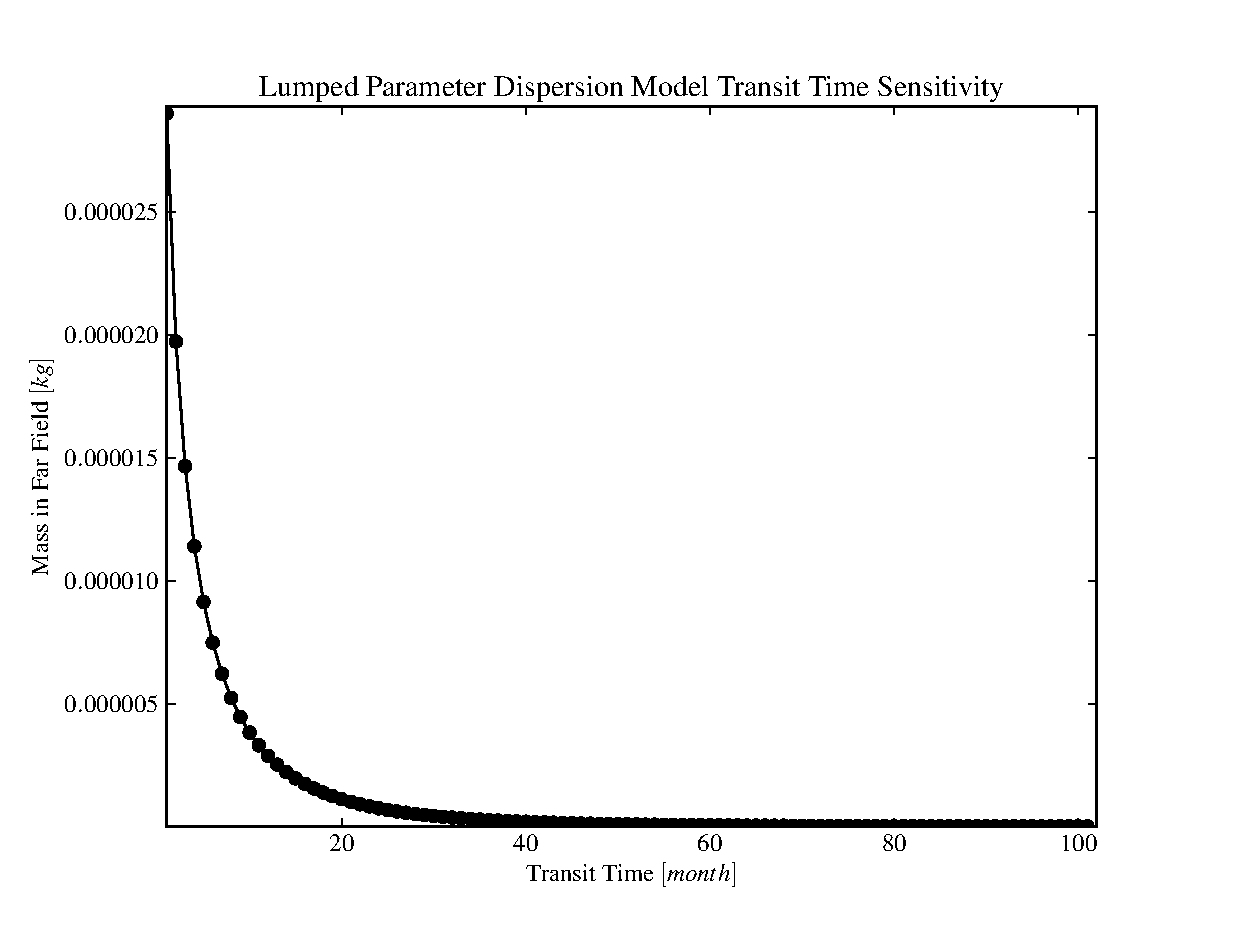
\includegraphics[width=0.8\textwidth]{./chapters/demonstration/base/lpDM_t_t.eps}
\caption[Lumped Parameter Dispersion Model Transit Time Sensitivity]{The transit time 
parameterization of the lumped parameter dispersion model of radionuclide 
transport has a strong effect on the material reaching the far field after 30 
years.  }
\label{fig:lp_t_t_begin}
\end{figure}
\end{frame}

\begin{frame}[ctb!]
\begin{figure}[ht]
\centering
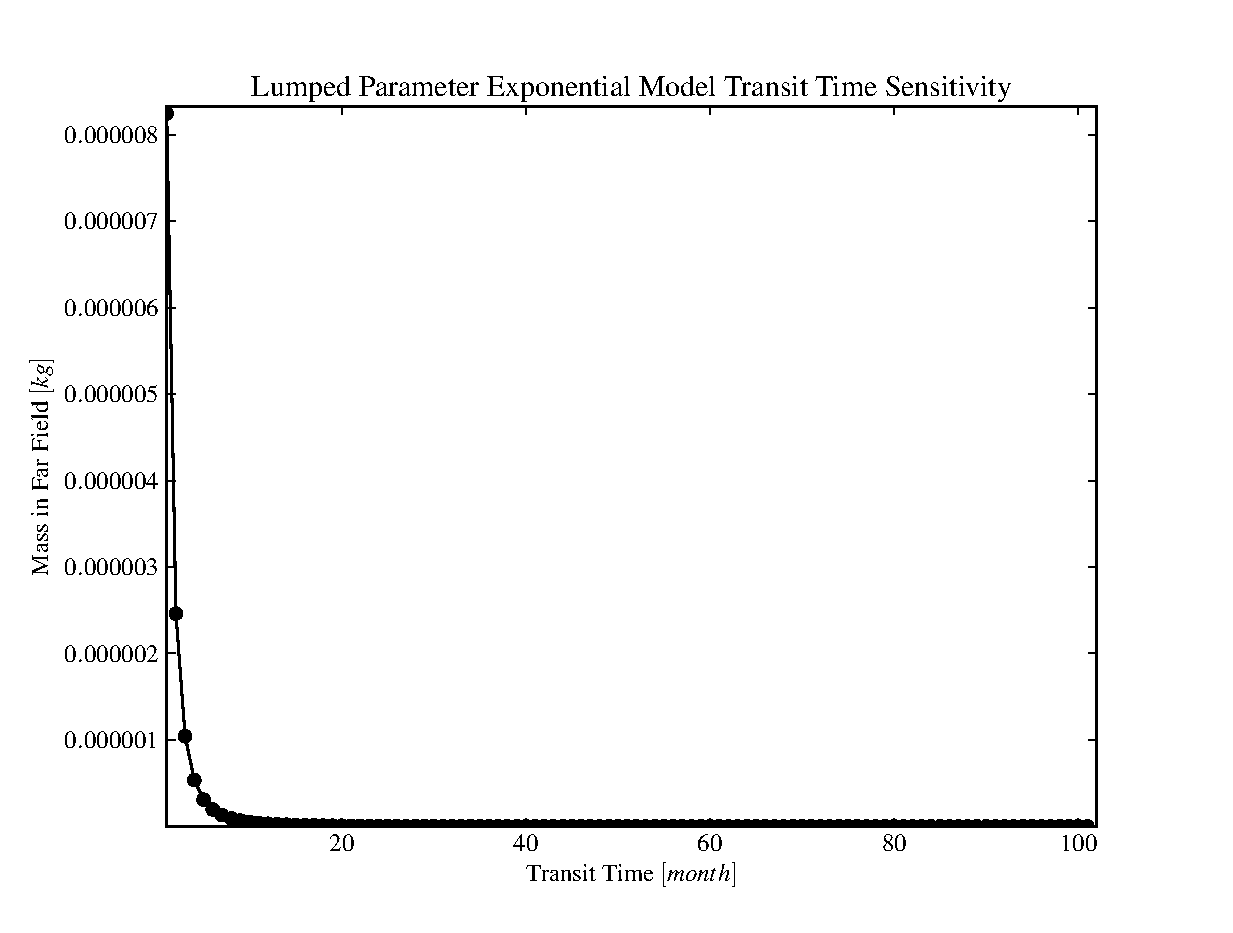
\includegraphics[width=0.8\textwidth]{./chapters/demonstration/base/lpEXPM_t_t.eps}
\caption[Lumped Parameter Exponential Model Transit Time Sensitivity]{The transit time 
parameterization of the lumped parameter exponential model of radionuclide 
transport has a strong effect on the material reaching the far field after 30 
years.  }
\end{figure}
\end{frame}

\begin{frame}[ctb!]
\begin{figure}[ht]
\centering
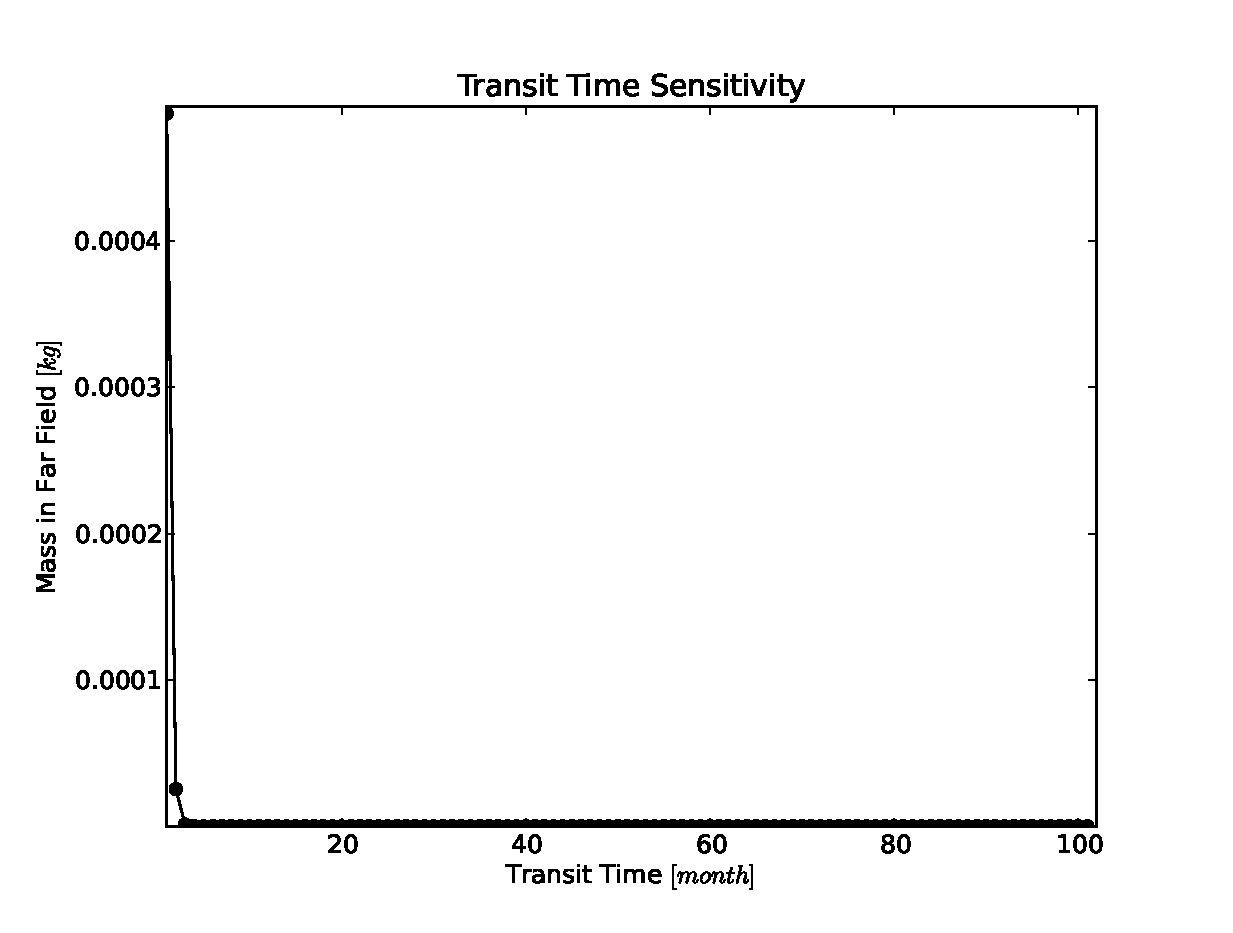
\includegraphics[width=0.8\textwidth]{./chapters/demonstration/base/lpPFM_t_t.eps}
\caption[Lumped Parameter Piston Flow Model Transit Time Sensitivity]{The transit time 
parameterization of the lumped parameter piston flow model of radionuclide 
transport has a strong effect on the material reaching the far field after 30 
years.  }
\label{fig:lp_t_t_end}
\end{figure}
\end{frame}

  \end{minipage}
\end{frame}

\subsection{Thermal Toy Cases}
\subsection{Radionuclide Toy Cases}
\subsection{Thermal Validation Cases}
\subsection{Radionuclide Validation Cases}


\begin{frame}[ctb!]
  \frametitle{Conclusion : Summary of Contributions}
\end{frame}

\begin{frame}[ctb!]
  \frametitle{Conclusion : Suggested Future Work}
\end{frame}


%%--------------------------------%%
%%--------------------------------%%
\begin{frame}[allowframebreaks]
  \frametitle{References}
  \bibliographystyle{plain}
  {\footnotesize \bibliography{ne571} }

\end{frame}

%%--------------------------------%%




\end{document}



